%% confbci tool paper, IEEE EMBC format.
%% Class used, in order of preference:
%%   1. ieeeconf.cls, the EMBC/PaperCept template class, if it sits next to this file;
%%   2. IEEEtran.cls in conference mode (part of every TeX Live and Overleaf), whose
%%      layout is the one ieeeconf.cls is derived from;
%%   3. a plain two-column article, only so the text can be checked.
\IfFileExists{ieeeconf.cls}{%
  \documentclass[letterpaper, 10pt, conference]{ieeeconf}
  \IEEEoverridecommandlockouts
  \overrideIEEEmargins
}{\IfFileExists{IEEEtran.cls}{%
  \documentclass[letterpaper, 10pt, conference]{IEEEtran}
  \IEEEoverridecommandlockouts
}{%
  \documentclass[letterpaper, 10pt, twocolumn]{article}
  \usepackage[margin=0.75in, columnsep=0.2in]{geometry}
  \usepackage{times}
}}
\usepackage{amsmath, amssymb}
\usepackage{graphicx}
\usepackage{booktabs}
\usepackage{xcolor}
\usepackage{url}

\newcommand{\dR}{\delta_R}

%% If the ieeeconf build spills onto page 5, first uncomment these three lines.
%% If it still does, delete the paragraph marked "R3-PER-GAMMA" in Sec. III-C AND
%% the abstract clause "and adaptive inference cut ... from 0.18 to 0.06", which
%% that paragraph is the only support for.
% \setlength{\textfloatsep}{8pt plus 2pt minus 2pt}
% \setlength{\abovecaptionskip}{3pt}
% \setlength{\belowcaptionskip}{0pt}

\title{\LARGE \bf confbci: Conformal Prediction Sets with Coverage Guarantees\\
for Motor-Imagery Brain--Computer Interfaces in Stroke Rehabilitation}

\author{Varun Bajpai$^{1}$%
\thanks{$^{1}$Independent researcher, Kanpur, India. \texttt{varunku3117p@gmail.com}. Code:
\protect\url{https://github.com/MACVXACE/confbci}.}}

\begin{document}
\maketitle
\thispagestyle{empty}
\pagestyle{empty}

\begin{abstract}
Motor-imagery brain--computer interfaces (BCIs) for stroke rehabilitation give
feedback on every trial, although cross-subject decoders are often near chance on
patients. We present \texttt{confbci}, an open-source Python toolkit that wraps a
decoder so that it returns a prediction set with a finite-sample coverage
guarantee and abstains when more than one label remains. It provides a
probabilistic Riemannian classifier, split, weighted, per-subject (Mondrian) and
adaptive conformal predictors, conformal risk control for the rate of wrong
feedback, and a leave-one-subject-out benchmark with zero-calibration, few-shot
and online regimes. On synthetic covariance matrices the coverage follows its
exact Beta law. On 50 acute stroke patients the decoder was near chance
(51--53\%). The conformal predictor met its 0.80 coverage target by abstaining
on about 60\% of trials, which cut wrong feedback from 49\% to 19\% of trials
but also cut correct feedback from 51\% to 20\%: the decisions it kept were
right only 53--56\% of the time. Re-centering raised the coverage of the worst
decile of patients from 0.50 to 0.64, and adaptive inference cut the
per-patient coverage error from 0.18 to 0.06. Weighted conformal prediction
was uninformative in the 435-dimensional tangent space: it either abstained on nearly every
trial or, under strong regularization, reduced to pooled calibration. Early
confidence did not predict later accuracy (Spearman $\rho=-0.036$, $p=0.80$). On
this data the toolkit's most useful output is quantified evidence that the
decoder should not gate feedback.
\end{abstract}

\section{INTRODUCTION}
BCI-driven neurofeedback is used in post-stroke motor rehabilitation on the
premise that feedback contingent on sensorimotor activity supports recovery
\cite{cervera2018}. The decoder therefore acts as a gate on reinforcement, and
feedback on a wrongly decoded trial rewards the wrong pattern. Decoders
nevertheless output a label on every trial. This matters most where they are
weakest: zero-calibration decoding of new patients, and the sizeable group of
users whose accuracy stays below about 70\% \cite{blankertz2010}.

Uncertainty estimates for motor-imagery decoders have been studied as heuristic
rejection rules \cite{uqmi2025}, which carry no guarantee. Conformal prediction
\cite{vovk2005,angelopoulos2023} turns any score into a prediction set that
contains the true label with probability at least $1-\alpha$, assuming only that
calibration and test trials are exchangeable. EEG violates that assumption in two
ways: between subjects, and within a session. Conformal methods have been
evaluated under cross-patient shift for seizure classification
\cite{eegconformal2026}; we are not aware of a toolkit or benchmark for
motor-imagery decoding in patients.

\texttt{confbci} contributes conformal predictors matched to each violation, a
benchmark that separates between-subject from within-session effects, a test
suite that checks each guarantee against its law, and results on 50 stroke
patients \cite{liu2024}.

\section{METHODS}
\subsection{Probabilistic minimum distance to mean}
Each trial is represented by its spatial covariance $C$, a symmetric positive
definite (SPD) matrix. With the affine-invariant distance
$\dR(A,B)=\|\log(A^{-1/2}BA^{-1/2})\|_F$ and Riemannian class means $M_k$
\cite{barachant2012},
\begin{equation}
p(y=k\mid C)=\frac{\exp(-\dR^2(C,M_k)/\tau)}{\sum_j \exp(-\dR^2(C,M_j)/\tau)} .
\end{equation}
The temperature $\tau$ minimizes the negative log-likelihood on a split held out
from the estimation of the $M_k$ (whole subjects when at least four are
available). Optional re-centering maps each subject $s$ with mean $\bar C_s$ to
$\tilde C=\bar C_s^{-1/2}C\,\bar C_s^{-1/2}$ \cite{zanini2018}; it uses no labels.
For a held-out patient, $\bar C_s$ is the mean of all 40 of that patient's
trials, including trials that come later in the session, so every re-centered
result below (Table~I; Fig.~2, right; R3) is transductive and an offline upper
bound on what a live system could achieve.

\subsection{Scores and split conformal prediction}
A nonconformity score $s(x,y)$ is larger when label $y$ fits trial $x$ worse. We
provide $s=1-p(y\mid x)$ and a geometric margin that needs no probability model,
\begin{equation}
s(C,y)=\dR(C,M_y)-\min_{k\neq y}\dR(C,M_k).
\end{equation}
Given $n$ calibration scores of the true labels, let $\hat q$ be their $r$-th
smallest value, $r=\lceil (n+1)(1-\alpha)\rceil$, and
$\mathcal C(x)=\{y: s(x,y)\le \hat q\}$. Under exchangeability
$1-\alpha\le P(Y\in\mathcal C(X))$, with $P(Y\in\mathcal C(X))\le 1-\alpha+1/(n+1)$
when scores have no ties. For i.i.d.\ continuous scores the coverage
conditional on the calibration set follows $\mathrm{Beta}(r,\,n+1-r)$
\cite{vovk2012}. For
two classes, $\mathcal C(x)$ with two labels is an abstention.

\subsection{Between-subject shift}
\emph{Weighted conformal prediction} \cite{tibshirani2019} replaces the empirical
quantile by that of the distribution placing mass $w_i/(\sum_j w_j+w(x))$ on
calibration score $i$ and $w(x)/(\sum_j w_j+w(x))$ at $+\infty$, where $w$ is the
density ratio between target and source. We estimate
$w(x)=(n_s/n_t)\,P(\mathrm{target}\mid x)/P(\mathrm{source}\mid x)$ with an
$\ell_2$-regularized logistic regression (inverse strength
$C\in\{10^{-1},\dots,10^{-4}\}$, default $10^{-1}$) on tangent-space vectors at
the global Riemannian mean, clip at the 99th percentile, and report the effective sample
size $(\sum w)^2/\sum w^2$ and $m_\infty$, the median over target trials of the
mass placed at $+\infty$. When that mass exceeds $\alpha$ the set is the full
label set.

\emph{Mondrian calibration} computes $\hat q$ separately for each subject from a
short labeled block of that subject, so the guarantee holds per subject and
requires exchangeability only within the subject. A block of $n$ trials gives a
finite threshold only if $n\ge 1/\alpha-1$, and its expected coverage is
$r/(n+1)$.

\subsection{Within-session shift: adaptive conformal inference}
In cued training the label is known when the trial ends. Adaptive conformal
inference \cite{gibbs2021} uses the quantile at a working level $\alpha_t$ and
updates
\begin{equation}
\alpha_{t+1}=\alpha_t+\gamma\,(\alpha-\mathrm{err}_t),\quad
\mathrm{err}_t=\mathbf 1\{y_t\notin\mathcal C_t(x_t)\},
\end{equation}
so a miss enlarges the next sets. For any sequence,
\begin{equation}
\left|\frac{1}{T}\sum_{t=1}^{T}\mathrm{err}_t-\alpha\right|\le
\frac{\max(\alpha_1,1-\alpha_1)+\gamma}{\gamma T}. \label{eq:aci}
\end{equation}

\subsection{Risk control for feedback}
Let feedback be given when the decoder's confidence
$\mathrm{conf}=\max_k p(k\mid C)$ is at least $\lambda$. The
loss $L(\lambda)=\mathbf 1\{\mathrm{conf}\ge\lambda\ \wedge\ \hat y\ne y\}$ is
bounded and non-increasing in $\lambda$, so conformal risk control
\cite{angelopoulos2024} applies: over a grid fixed in advance we take the smallest
$\lambda$ with $\tfrac{n}{n+1}\hat R(\lambda)+\tfrac{1}{n+1}\le\alpha$, which gives
$P(\text{feedback given}\wedge\text{wrong})\le\alpha$ under exchangeability while
giving feedback as often as the constraint allows.

\subsection{Evaluation regimes}
One subject is held out at a time. \textbf{R1 (zero calibration):} the remaining
subjects are split by subject into training and calibration subjects; we compare
pooled split, weighted, and re-centered split conformal prediction. \textbf{R2
(few-shot):} the first $k\in\{2,4,8\}$ trials per class of the target form a
Mondrian calibration block and the rest are tested, once in recorded order and
once with a randomly drawn block. The random draw is exchangeable by
construction, so the difference between orders measures within-session
non-stationarity. \textbf{R3 (online):} trials are replayed in order through
adaptive conformal inference, started from the calibration subjects' scores,
with $\gamma\in\{0.005,0.01,0.05\}$. \textbf{Screening:} a threshold from source
subjects is applied to the first $b=20$ unlabeled trials of the target; the
fraction of singleton sets is compared with accuracy on the remaining trials by
Spearman's $\rho$ and by the AUROC for accuracy $\ge 70\%$, with bootstrap
intervals over patients.

\subsection{Data and implementation}
Covariances (OAS shrinkage, 8--32\,Hz) are obtained through MOABB
\cite{jayaram2018} for the acute-stroke dataset of Liu \emph{et al.}
\cite{liu2024}: 50 patients, left- versus right-hand imagery, 29 channels
(tangent dimension $c(c+1)/2=435$), 40 trials per patient. We use
$\alpha=0.2$ and the margin score (2) for all patient results. With 40 trials, regime R2 is evaluated for $k\le 8$; the next doubling
($k=16$) leaves fewer than ten test trials. The package depends on NumPy, SciPy,
scikit-learn and pyRiemann;
237 unit tests run on synthetic SPD matrices drawn from a wrapped Gaussian on the
manifold.

\section{RESULTS}
\subsection{Validation on synthetic data}
Over 1{,}000 random calibration sets, coverage matched $\mathrm{Beta}(r,\,n+1-r)$ in
all twelve settings ($n\in\{50,99,400\}$, $\alpha\in\{0.1,0.2\}$, two scores;
smallest Kolmogorov--Smirnov $p=0.055$; Fig.~\ref{fig:beta}). Two incorrect
quantile rules failed the same test ($p<10^{-9}$). Under a known covariate shift,
weighted conformal prediction with estimated weights was within 0.03 of target.
Risk control at
$\alpha=0.10$ ($n=200$) gave a joint wrong-feedback rate of 0.099 with feedback
on 61\% of trials.

\begin{figure}[t]
\centering
\IfFileExists{figures/fig_beta_validity.pdf}{%
  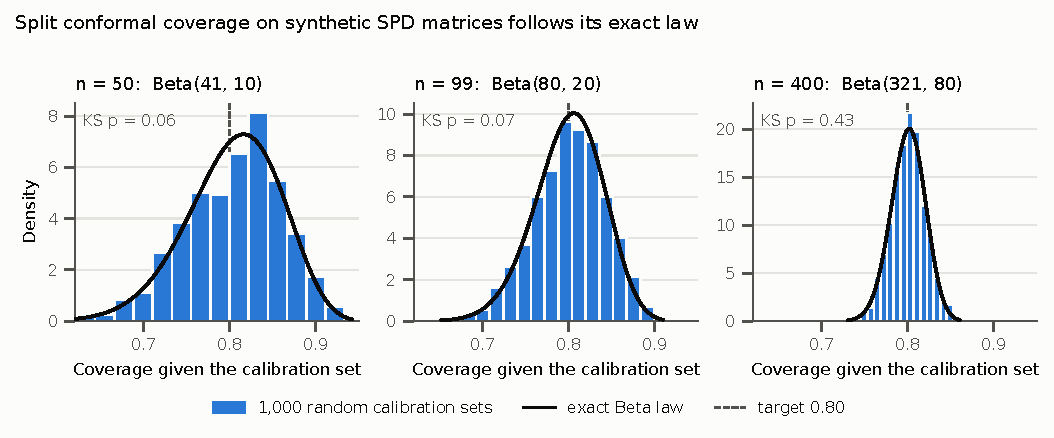
\includegraphics[width=\columnwidth]{figures/fig_beta_validity.pdf}}{%
  \fbox{\parbox[c][2.2cm][c]{0.9\columnwidth}{\centering run \texttt{benchmarks/make\_figures.py}}}}
\caption{Split conformal coverage conditional on the calibration set, over
1{,}000 random calibration sets of synthetic SPD matrices ($1-p$ score,
$\alpha=0.2$), against the exact laws $\mathrm{Beta}(41,10)$,
$\mathrm{Beta}(80,20)$ and $\mathrm{Beta}(321,80)$ for $n=50,99,400$: three of
the twelve settings in Sec.~III-A. Titles give the Kolmogorov--Smirnov $p$;
density scales differ between panels.}
\label{fig:beta}
\end{figure}

\subsection{Zero calibration on stroke patients (R1)}
Table~\ref{tab:r1} summarizes the 50 held-out patients. Weighted conformal
prediction was uninformative. The domain classifier separated each target from
the calibration subjects almost perfectly, the median mass at $+\infty$ was
$\approx 0.95>\alpha$, and the method therefore returned the full label set on
nearly every trial (singleton rate 0.014). This is valid and gives no
decisions. Stronger regularization did not rescue the method; it moved it
toward pooled calibration. At $C=10^{-2}$ the mass at $+\infty$ was still 0.66
and the sets were unchanged; at $C=10^{-3}$ it fell to 0.075, with coverage 0.86
and singleton rate 0.29; at $C=10^{-4}$ it was 0.004, with coverage 0.805 and
singleton rate 0.40, essentially the pooled result (0.814, 0.39). With 435
tangent dimensions and 40 target trials, the weights are either too sharp to
leave calibration mass or too flat to correct anything. We did not record the
worst-decile coverage of the sweep.

Pooled and re-centered split conformal prediction both reached the target on
average (0.814, 0.808) and differ in the tail: the worst decile of patients
was covered at 0.500 with pooling and 0.635 with re-centering, and the share of
patients more than 0.05 below target fell from 34\% to 26\%. With 40 test
trials per patient, binomial noise alone would put the worst decile at about
0.69 for a predictor that covers every patient at exactly 0.80, so re-centering
removes most, not all, of the patient-level under-coverage.

The sets are valid and of little practical use at this accuracy. Both methods
abstained on about 60\% of trials, and on the trials where they committed the
decoded label was right 53\% (pooled) and 56\% (re-centered) of the time,
averaged over patients. Decoder accuracy on all trials was 51.4\% and 52.5\%. A
decoder that always commits therefore gives wrong feedback on 48.6\% (pooled)
and 47.5\% (re-centered) of trials; the conformal predictor gave it on 18.5\%
and 19.2\% (Table~I). It also gave correct feedback on only 20.4\% and 23.2\%
of trials, against 51.4\% and 52.5\%.
Abstention reduced how often the patient would be misled without making the
feedback that remained more trustworthy. A wrong-feedback rate of 0.19 is what
$\alpha=0.2$ permits for a two-class decoder at chance: it commits on about
$2\alpha$ of trials and is wrong on half.

\begin{table}[t]
\caption{Regime R1 on 50 stroke patients, $\alpha=0.2$ (target coverage 0.80).
Cov.: mean coverage; Worst 10\%: mean coverage of the worst decile of patients;
Singl.: share of trials with a one-label set (feedback given); Wrong fb.:
share of all trials with feedback given and wrong; Sel.\ acc.: accuracy on
singleton trials.}
\label{tab:r1}
\centering
\small\setlength{\tabcolsep}{3pt}
\begin{tabular}{@{}lccccc@{}}
\toprule
Method & Cov. & Worst 10\% & Singl. & Wrong fb. & Sel.\ acc. \\
\midrule
Pooled CP & 0.814 & 0.500 & 0.389 & 0.185 & 0.535 \\
Weighted CP & 0.993 & 0.925 & 0.014 & 0.008 & 0.461 \\
Re-centered CP & 0.808 & 0.635 & 0.424 & 0.192 & 0.559 \\
\bottomrule
\end{tabular}
\end{table}

\subsection{Few-shot and online regimes (R2, R3)}
In R2, chronological Mondrian calibration gave mean coverages of 0.816, 0.895
and 0.839 for $k=2,4,8$, against 0.800, 0.889 and 0.824 expected under
exchangeability; a randomly drawn block gave 0.834, 0.895 and 0.832
(Fig.~\ref{fig:r2}, left). With the re-centered decoder (right) the two orders
gave 0.807, 0.884, 0.816 and 0.798, 0.897, 0.826. In both panels the orders
differ by less than 0.02 at every $k$, within
the standard error of the chronological mean (about 0.02--0.03 over 50
patients).

%% R3-PER-GAMMA (first paragraph to cut if over 4 pages; ends at "more often right.")
In R3, the mean per-patient long-run coverage error was 0.179 with a static
threshold and 0.161, 0.148 and 0.061 with adaptive inference at
$\gamma=0.005, 0.01, 0.05$; binomial noise alone gives about 0.05 at 40 trials.
At $\gamma=0.05$ the coverage of the worst decile of patients rose from 0.50 to
0.71 and the share under-covered fell from 34\% to 24\%, but accuracy on committed trials
fell from 53\% to 47\%: adaptation spread the coverage more evenly over
patients without making the decisions it committed to more often right.
The mean minimum rolling 20-trial coverage was 0.775 (static) and 0.732
(adaptive, $\gamma=0.05$), and 0.746 and 0.737 with the non-causal re-centered
decoder, so adaptation did not improve the worst window. With 40 trials, bound~(\ref{eq:aci}) is 0.425 at $\gamma=0.05$, so this is an
empirical observation (limitation 1).

\begin{figure}[t]
\centering
\IfFileExists{figures/fig_r2_coverage.pdf}{%
  \includegraphics[width=\columnwidth]{figures/fig_r2_coverage.pdf}}{%
  \fbox{\parbox[c][2.2cm][c]{0.9\columnwidth}{\centering run \texttt{make\_figures.py --records results/Liu2024\_records.csv}}}}
\caption{Mean coverage over 50 patients against calibration block size $k$ in
regime R2, for the plain (left) and re-centered (right) decoder, with the block
in recorded order (chronological) or drawn at random (shuffled; 20 draws per
patient). Dotted: coverage expected under exchangeability,
$r/(n+1)$ with $n=2k$, whose saw-tooth shape comes from the ceiling in $r$, not
from the data; dashed: target 0.80.}
\label{fig:r2}
\end{figure}

\subsection{Patient screening}
The singleton rate on the initial block did not predict held-out accuracy:
Spearman $\rho=-0.036$, $p=0.80$, $n=50$ (95\% bootstrap interval
$[-0.309, 0.239]$). The AUROC for accuracy $\ge 70\%$ was 0.321 (95\% bootstrap
interval $[0.147, 0.521]$), with 8 of 50
patients at or above the threshold; with 8 against 42 patients the standard
error of an AUROC under no association is about 0.11, so this is not
distinguishable from 0.5. On 20 held-out
trials a chance-level decoder reaches 70\% with probability 0.058, so about
three of the eight are expected by chance alone.

\section{DISCUSSION}
Two findings stand out. First, importance weighting in
the tangent space is the wrong tool for subject shift at this sample size: the
dimension exceeds the number of target trials, and across four orders of
magnitude of regularization the method either abstained or reproduced pooled
calibration. A lower-dimensional shift representation would be needed. Second, marginal validity across patients did not require
any correction: pooled calibration on held-out subjects already averaged 0.81.
What pooling got wrong was the distribution over patients, and re-centering
\cite{zanini2018} and online adaptation each reduced that patient-level error.

A coverage guarantee is not a usefulness guarantee. At 51\% accuracy the
predictor met its target by abstaining on most trials and committing, nearly at
random, on the rest. That is the intended behavior: given a decoder that cannot
separate the classes, a valid predictor withholds feedback on most trials and
states how often it will still be wrong. It cannot create accuracy the decoder
lacks. For a rehabilitation system the informative outputs are
therefore the abstention rate and the accuracy on committed trials, and a
decoder at this level should not be used to gate feedback at any $\alpha$.

The screening result is a null and should be read as inconclusive. It does not
show that early confidence and later accuracy are unrelated, and by itself it
says nothing about non-stationarity. At least three explanations fit it. (a)
\emph{Restricted range:} if cross-subject accuracy is near chance for most
patients, as the mean of 51--53\% in R1 suggests, there is little between-patient
variance to predict. (b) \emph{Measurement noise:} accuracy on $m$ held-out
trials has standard error $\sqrt{0.25/m}$, i.e.\ 0.11 for $m=20$, comparable to
the between-patient spread; the singleton rate on 20 trials is equally coarse.
With $n=50$ the interval on $\rho$ still admits correlations of roughly
$\pm 0.3$. (c) \emph{Non-stationarity} between the block and the rest of the
session. The quantity that tests (c) directly is the chronological-versus-shuffled
gap in R2, which holds the patient and the decoder fixed. That gap was below
0.02 at every $k$, so these data give no evidence of within-session
non-stationarity of the scores, although gaps smaller than about 0.05 cannot be
excluded. Explanations (a) and (b) are therefore the more likely ones. A
screening test would have to be evaluated on a decoder with above-chance
accuracy and with longer sessions.

\subsection{Limitations}
\emph{(1) The online guarantee is a long-run average and is vacuous for short
sessions.} Bound~(\ref{eq:aci}) decays as $1/(\gamma T)$. For $T=40$ trials and
$\gamma=0.05$ it equals 0.425, and 0.07 for $T=240$; it does not constrain the
coverage of any single trial or 20-trial window. On sessions of the present
length, coverage under adaptive inference is an empirical observation, not a
consequence of the bound.

\emph{(2) Risk control bounds a joint rate.} The guarantee is
$P(\text{feedback given}\wedge\text{wrong})\le\alpha$ per trial attempted, in
expectation over calibration sets. The error rate among trials that receive
feedback is larger by the factor $1/P(\text{feedback})$ (0.099/0.61 $\approx$ 16\%
in the synthetic example) and is not bounded here.

\emph{(3) All re-centered results are transductive offline upper bounds.}
Re-centering uses the mean of all 40 of a patient's trials, including future
ones, which a live system cannot do. This applies to every re-centered result:
the re-centered row of Table~I, the right panel of Fig.~2, and the re-centered
static and adaptive results in R3. A causal reference, estimated from an
initial block and updated as trials arrive, is not yet implemented.

Further limits: coverage is marginal, not conditional on class; risk control
was validated on synthetic data only and not run on the patients; results are
offline replays of one dataset, one decoder family and one setting of $\alpha$;
and no patient received feedback from this system, so no clinical benefit is
claimed.

\section{CONCLUSION}
\texttt{confbci} makes abstention with stated guarantees available for
motor-imagery decoders and measures where those guarantees stop holding. On 50
stroke patients, average coverage held without calibration data from the
patient, re-centering and online adaptation reduced patient-level coverage
error, importance weighting either abstained or reduced to pooling, and a short unlabeled block did not
identify which patients would decode well. With decoding near chance, the main
practical output of the predictor was the instruction to abstain.

\section*{ACKNOWLEDGMENT}
The author conceived the study, designed the experimental benchmarks, ran all
analyses on the patient data, and verified every reported result. Anthropic's
Claude was used as an assistive tool during software implementation and
manuscript drafting.

\footnotesize
\begin{thebibliography}{99}
\bibitem{cervera2018} M. A. Cervera \emph{et al.}, ``Brain-computer interfaces
for post-stroke motor rehabilitation: a meta-analysis,'' \emph{Ann. Clin. Transl.
Neurol.}, vol. 5, no. 5, pp. 651--663, 2018.
\bibitem{blankertz2010} B. Blankertz \emph{et al.}, ``Neurophysiological
predictor of SMR-based BCI performance,'' \emph{NeuroImage}, vol. 51, no. 4,
pp. 1303--1309, 2010.
\bibitem{uqmi2025} J. Suurmeijer, I. P. de Jong, and M. Valdenegro-Toro, ``Uncertainty quantification for motor
imagery BCI -- machine learning vs. deep learning,'' arXiv:2507.07511, 2025.
\bibitem{vovk2005} V. Vovk, A. Gammerman, and G. Shafer, \emph{Algorithmic
Learning in a Random World}. Springer, 2005.
\bibitem{angelopoulos2023} A. N. Angelopoulos and S. Bates, ``Conformal
prediction: a gentle introduction,'' \emph{Found. Trends Mach. Learn.}, vol. 16,
no. 4, pp. 494--591, 2023.
\bibitem{eegconformal2026} A. Chatterjee \emph{et al.}, ``Making conformal predictors robust
in healthcare settings: a case study on EEG classification,'' arXiv:2602.19483,
2026.
\bibitem{liu2024} H. Liu \emph{et al.}, ``An EEG motor imagery dataset for brain
computer interface in acute stroke patients,'' \emph{Sci. Data}, vol. 11,
art. 131, 2024.
\bibitem{barachant2012} A. Barachant, S. Bonnet, M. Congedo, and C. Jutten,
``Multiclass brain-computer interface classification by Riemannian geometry,''
\emph{IEEE Trans. Biomed. Eng.}, vol. 59, no. 4, pp. 920--928, 2012.
\bibitem{zanini2018} P. Zanini, M. Congedo, C. Jutten, S. Said, and
Y. Berthoumieu, ``Transfer learning: a Riemannian geometry framework with
applications to brain-computer interfaces,'' \emph{IEEE Trans. Biomed. Eng.},
vol. 65, no. 5, pp. 1107--1116, 2018.
\bibitem{vovk2012} V. Vovk, ``Conditional validity of inductive conformal
predictors,'' in \emph{Proc. Asian Conf. Mach. Learn.}, 2012, pp. 475--490.
\bibitem{tibshirani2019} R. J. Tibshirani, R. F. Barber, E. J. Cand\`es, and
A. Ramdas, ``Conformal prediction under covariate shift,'' in \emph{Adv. Neural
Inf. Process. Syst.}, vol. 32, 2019.
\bibitem{gibbs2021} I. Gibbs and E. J. Cand\`es, ``Adaptive conformal inference
under distribution shift,'' in \emph{Adv. Neural Inf. Process. Syst.}, vol. 34,
2021.
\bibitem{angelopoulos2024} A. N. Angelopoulos, S. Bates, A. Fisch, L. Lei, and
T. Schuster, ``Conformal risk control,'' in \emph{Proc. Int. Conf. Learn.
Represent.}, 2024.
\bibitem{jayaram2018} V. Jayaram and A. Barachant, ``MOABB: trustworthy
algorithm benchmarking for BCIs,'' \emph{J. Neural Eng.}, vol. 15, no. 6,
066011, 2018.
\end{thebibliography}

\end{document}
